%%%%%%%%%%%%%%%%%%%%%%%%%%%%%%%%%%%%%%%%%%%%%%%%%%%%%%%%%%%%%%%%%%%%%%%%%%%%%%%%%
% Template: Exam
%
% Por: Abrantes Araújo Silva Filho
%      abrantesasf@gmail.com
%
% Citação: Se você gostou deste template, por favor ajude a divulgá-lo mantendo
%          o link para meu repositório GitHub em:
%          https://github.com/abrantesasf/LaTeX
%%%%%%%%%%%%%%%%%%%%%%%%%%%%%%%%%%%%%%%%%%%%%%%%%%%%%%%%%%%%%%%%%%%%%%%%%%%%%%%%%




%%%%%%%%%%%%%%%%%%%%%%%%%%%%%%%%%%%%%%%%%%%%%%%%%%%%%%%%%%%%%%%%%%%%%%%%%%%%%%%%%
%%% Configura o tipo de documento, papel, tamanho da fonte e informações básicas
%%% para as proriedades do PDF/DVIPS e outras propriedades do documento
\RequirePackage{ifpdf}
\ifpdf
  % Classe, língua e tamanho da fonte padrão. Outras opções a considerar:
  %   draft
  %   onecolumn (padrão) ou twocolumn (OU usar o package multicol)
  %   fleqn com ou sem leqno (alinhamento à esquerda das fórmulas e dos números)
  %   oneside (padrão para article ou report) ou twoside (padrão para book)
  %   answers = imprime respostas para o gabarito
  \documentclass[pdftex, brazil, 12pt, oneside, addpoints]{exam}
\else
  % Classe, língua e tamanho da fonte padrão. Outras opções a considerar:
  %   draft
  %   onecolumn (padrão) ou twocolumn (OU usar o package multicol)
  %   fleqn com ou sem leqno (alinhamento à esquerda das fórmulas e dos números)
  %   oneside (padrão para article ou report) ou twoside (padrão para book)
  %   answers = imprime respostas para o gabarito
  \documentclass[brazil, 12pt, oneside, addpoints]{exam}
\fi


%%%%%%%%%%%%%%%%%%%%%%%%%%%%%%%%%%%%%%%%%%%%%%%%%%%%%%%%%%%%%%%%%%%%%%%%%%%%%%%%%
%%% Carrega pacotes iniciais necessários para estrutura de controle e para a
%%% criação e o parse de novos comandos
\usepackage{ifthen}
\usepackage{xparse}


%%%%%%%%%%%%%%%%%%%%%%%%%%%%%%%%%%%%%%%%%%%%%%%%%%%%%%%%%%%%%%%%%%%%%%%%%%%%%%%%%
%%% Configuração do tamanho da página, margens, espaçamento entrelinhas e, se
%%% necessário, ativa a indentação dos primeiros parágrafos.
\ifpdf
  \usepackage[pdftex]{geometry}
\else
  \usepackage[dvips]{geometry}
\fi
\geometry{a4paper, left=2.0cm, right=2.0cm, top=2.0cm, bottom=2.0cm}

\usepackage{setspace}
  \singlespacing
  %\onehalfspacing
  %\doublespacing


%%%%%%%%%%%%%%%%%%%%%%%%%%%%%%%%%%%%%%%%%%%%%%%%%%%%%%%%%%%%%%%%%%%%%%%%%%%%%%%%%
%%% Configurações de encoding, lingua e fontes:
\usepackage[T1]{fontenc}
\usepackage[utf8]{inputenc}
\usepackage{babel}

% Altera a fonte padrão do documento (nem todas funcionam em modo math):
%   phv = Helvetica
%   ptm = Times
%   ppl = Palatino
%   pbk = bookman
%   pag = AdobeAvantGarde
%   pnc = Adobe NewCenturySchoolBook
\renewcommand{\familydefault}{ppl}


%%%%%%%%%%%%%%%%%%%%%%%%%%%%%%%%%%%%%%%%%%%%%%%%%%%%%%%%%%%%%%%%%%%%%%%%%%%%%%%%%
%%% Configurações de cabeçalho e rodapé (não pode usar fancyhdr pois ocorre conflito):
\pagestyle{headandfoot}
\runningheadrule
\firstpageheader{}{}{}
\runningheader{Atividade de Recuperação da Aprendizagem}{}{Outubro/2018}
\firstpagefooter{}{}{Página \thepage\ de \numpages}
\runningfooter{}{}{Página \thepage\ de \numpages}
\runningfootrule


%%%%%%%%%%%%%%%%%%%%%%%%%%%%%%%%%%%%%%%%%%%%%%%%%%%%%%%%%%%%%%%%%%%%%%%%%%%%%%%%%
%%% Carrega pacotes para referências cruzadas, citações dentro do documento,
%%% links para internet e outros.Configura algumas opções.
%%% Não altere a ordem de carregamento dos packages.
\usepackage{varioref}
\ifpdf
  \usepackage[pdftex]{hyperref}
    \hypersetup{
      % Informações variáveis em cada documento (MUDE AQUI!):
      pdftitle={Atividade de Recuperação da Aprendizagem},
      pdfauthor={Prof.\ Rober Marconi},
      pdfsubject={Matrizes e Sistemas de Equações Lineares},
      pdfkeywords={matrizes, conceitos, operações, sistemas de equações lineares},
      pdfinfo={
        CreationDate={}, % Ex.: D:AAAAMMDDHH24MISS
        ModDate={}       % Ex.: D:AAAAMMDDHH24MISS
      },
      % Coisas que você não deve alterar se não souber o que está fazendo:
      unicode=true,
      pdflang={pt-BR},
      bookmarksopen=true,
      bookmarksnumbered=true,
      bookmarksopenlevel=5,
      pdfdisplaydoctitle=true,
      pdfpagemode=UseOutlines,
      pdfstartview=FitH,
      pdfcreator={LaTeX with hyperref package},
      pdfproducer={pdfTeX},
      pdfnewwindow=true,
      colorlinks=true,
      citecolor=green,
      linkcolor=red,
      filecolor=cyan,
      urlcolor=blue
    }
\else
  \usepackage{hyperref}
\fi
\usepackage{cleveref}
\usepackage{url}


%%%%%%%%%%%%%%%%%%%%%%%%%%%%%%%%%%%%%%%%%%%%%%%%%%%%%%%%%%%%%%%%%%%%%%%%%%%%%%%%%
%%% Carrega bibliotecas de símbolos (matemáticos, físicos, etc.), fontes
%%% adicionais, e configura algumas opções
\usepackage{amsmath}
\usepackage{amssymb}
\usepackage{amsfonts}
\usepackage{siunitx}
  \sisetup{group-separator = {.}}
  \sisetup{group-digits = {false}}
  \sisetup{output-decimal-marker = {,}}
\usepackage{bm}
\usepackage{cancel}
% Altera separador decimal via comando, se necessário (prefira o siunitx):
%\mathchardef\period=\mathcode`.
%\DeclareMathSymbol{.}{\mathord}{letters}{"3B}
  

%%%%%%%%%%%%%%%%%%%%%%%%%%%%%%%%%%%%%%%%%%%%%%%%%%%%%%%%%%%%%%%%%%%%%%%%%%%%%%%%%
%%% Carrega packages relacionados à computação
\usepackage{algorithm2e}
\usepackage{algorithmicx}
\usepackage{algpseudocode}
\usepackage{listings}
  \lstset{literate=
    {á}{{\'a}}1 {é}{{\'e}}1 {í}{{\'i}}1 {ó}{{\'o}}1 {ú}{{\'u}}1
    {Á}{{\'A}}1 {É}{{\'E}}1 {Í}{{\'I}}1 {Ó}{{\'O}}1 {Ú}{{\'U}}1
    {à}{{\`a}}1 {è}{{\`e}}1 {ì}{{\`i}}1 {ò}{{\`o}}1 {ù}{{\`u}}1
    {À}{{\`A}}1 {È}{{\'E}}1 {Ì}{{\`I}}1 {Ò}{{\`O}}1 {Ù}{{\`U}}1
    {ä}{{\"a}}1 {ë}{{\"e}}1 {ï}{{\"i}}1 {ö}{{\"o}}1 {ü}{{\"u}}1
    {Ä}{{\"A}}1 {Ë}{{\"E}}1 {Ï}{{\"I}}1 {Ö}{{\"O}}1 {Ü}{{\"U}}1
    {â}{{\^a}}1 {ê}{{\^e}}1 {î}{{\^i}}1 {ô}{{\^o}}1 {û}{{\^u}}1
    {Â}{{\^A}}1 {Ê}{{\^E}}1 {Î}{{\^I}}1 {Ô}{{\^O}}1 {Û}{{\^U}}1
    {œ}{{\oe}}1 {Œ}{{\OE}}1 {æ}{{\ae}}1 {Æ}{{\AE}}1 {ß}{{\ss}}1
    {ű}{{\H{u}}}1 {Ű}{{\H{U}}}1 {ő}{{\H{o}}}1 {Ő}{{\H{O}}}1
    {ç}{{\c c}}1 {Ç}{{\c C}}1 {ø}{{\o}}1 {å}{{\r a}}1 {Å}{{\r A}}1
    {€}{{\euro}}1 {£}{{\pounds}}1 {«}{{\guillemotleft}}1
    {»}{{\guillemotright}}1 {ñ}{{\~n}}1 {Ñ}{{\~N}}1 {¿}{{?`}}1
  }
  

%%%%%%%%%%%%%%%%%%%%%%%%%%%%%%%%%%%%%%%%%%%%%%%%%%%%%%%%%%%%%%%%%%%%%%%%%%%%%%%%%
%%% Ativa suporte extendido a cores
\usepackage[svgnames]{xcolor} % Opções de cores: usenames (16), dvipsnames (64),
                              % svgnames (150) e x11names (300).


%%%%%%%%%%%%%%%%%%%%%%%%%%%%%%%%%%%%%%%%%%%%%%%%%%%%%%%%%%%%%%%%%%%%%%%%%%%%%%%%%
%%% Suporte à importação de gráficos externos
\ifpdf
  \usepackage[pdftex]{graphicx}
\else
  \usepackage[dvips]{graphicx}
\fi


%%%%%%%%%%%%%%%%%%%%%%%%%%%%%%%%%%%%%%%%%%%%%%%%%%%%%%%%%%%%%%%%%%%%%%%%%%%%%%%%%
%%% Suporte à criação de gráficos proceduralmente na LaTeX:
\usepackage{tikz}
  \usetikzlibrary{arrows,automata,backgrounds,matrix,patterns,positioning,shapes,shadows}


%%%%%%%%%%%%%%%%%%%%%%%%%%%%%%%%%%%%%%%%%%%%%%%%%%%%%%%%%%%%%%%%%%%%%%%%%%%%%%%%%
%%% Packages para tabelas
\usepackage{array}
\usepackage{longtable}
\usepackage{tabularx}
\usepackage{tabu}
\usepackage{lscape}
\usepackage{colortbl}  
\usepackage{booktabs}
\newcolumntype{M}[1]{>{\centering\arraybackslash}m{#1}}
%\newcolumntype{ML}[1]{>{$}l<{$}}
%\newcolumntype{MR}[1]{>{R}r<{R}}
\newcolumntype{L}[1]{>{\arraybackslash}m{#1}}
\newcolumntype{N}{@{}m{0pt}@{}}


%%%%%%%%%%%%%%%%%%%%%%%%%%%%%%%%%%%%%%%%%%%%%%%%%%%%%%%%%%%%%%%%%%%%%%%%%%%%%%%%%
%%% Packages ambientes de listas
\usepackage{enumitem}
\usepackage[ampersand]{easylist}


%%%%%%%%%%%%%%%%%%%%%%%%%%%%%%%%%%%%%%%%%%%%%%%%%%%%%%%%%%%%%%%%%%%%%%%%%%%%%%%%%
%%% Packages para suporte a ambientes floats, captions, etc.:
\usepackage{float}
\usepackage{wrapfig}
\usepackage{placeins}
\usepackage{caption}
\usepackage{sidecap}
\usepackage{subcaption}


%%%%%%%%%%%%%%%%%%%%%%%%%%%%%%%%%%%%%%%%%%%%%%%%%%%%%%%%%%%%%%%%%%%%%%%%%%%%%%%%%
%%% Meus comandos específicos:
% Commando para ``italizar´´ palavras em inglês (e outras línguas!):
\newcommand{\ingles}[1]{\textit{#1}}

% Commando para colocar o espaço correto entre um número e sua unidade:
\newcommand{\unidade}[2]{\ensuremath{#1\,\mathrm{#2}}}
\newcommand{\unidado}[2]{{#1}\,{#2}}

% Produz ordinal masculino ou feminino dependendo do segundo argumento:
\newcommand{\ordinal}[2]{%
#1%
\ifthenelse{\equal{a}{#2}}%
{\textordfeminine}%
{\textordmasculine}}


%%%%%%%%%%%%%%%%%%%%%%%%%%%%%%%%%%%%%%%%%%%%%%%%%%%%%%%%%%%%%%%%%%%%%%%%%%%%%%%%%
%%% Hifenização específica quando o LaTeX/Babel não conseguirem hifenizar:
\babelhyphenation{Git-Hub}


%%%%%%%%%%%%%%%%%%%%%%%%%%%%%%%%%%%%%%%%%%%%%%%%%%%%%%%%%%%%%%%%%%%%%%%%%%%%%%%%%
%%% Comandos específicos para a classe EXAM deste documento:
\newcommand{\umalinha}{\fillwithlines{0.25in}}
\newcommand{\duaslinhas}{\fillwithlines{0.50in}}
\newcommand{\treslinhas}{\fillwithlines{0.75in}}
\newcommand{\quatrolinhas}{\fillwithlines{1.00in}}
\newcommand{\cincolinhas}{\fillwithlines{1.25in}}
\newcommand{\seislinhas}{\fillwithlines{1.50in}}
\newcommand{\setelinhas}{\fillwithlines{1.75in}}
\newcommand{\oitolinhas}{\fillwithlines{2.00in}}
\newcommand{\novelinhas}{\fillwithlines{2.25in}}
\newcommand{\dezlinhas}{\fillwithlines{2.50in}}

% Verdadeiro ou Falvo para a classe EXAM
\newcommand{\vf}[1][{}]{%
  \fillin[#1][0.25in]%
}

% Título das respostas:
%\renewcommand{\solutiontitle}{\noindent\textbf{Resposta:}\par\noindent}
\renewcommand{\solutiontitle}{\noindent}
%\shadedsolutions
%\SolutionEmphasis{\itshape}




%%%%%%%%%%%%%%%%%%%%%%%%%%%%%%%%%%%%%%%%%%%%%%%%%%%%%%%%%%%%%%%%%%%%%%%%%%%%%%%%%
%%%%%%%%%%%%%%%%%%%%%%%%%%%%%%%%%%%%%%%%%%%%%%%%%%%%%%%%%%%%%%%%%%%%%%%%%%%%%%%%%
%%%%%%%%%%%%%%%%%%%%%%%%%%%%%%%%%%%%%%%%%%%%%%%%%%%%%%%%%%%%%%%%%%%%%%%%%%%%%%%%%
%%%%%%%%%%%%%%%%%%%%%%%%%%%%%%%%%%%%%%%%%%%%%%%%%%%%%%%%%%%%%%%%%%%%%%%%%%%%%%%%%
%%%%%%%%%%%%%%%%%%%%%%%%%%%%%% COMEÇA O DOCUMENTO %%%%%%%%%%%%%%%%%%%%%%%%%%%%%%%
%%%%%%%%%%%%%%%%%%%%%%%%%%%%%%%%%%%%%%%%%%%%%%%%%%%%%%%%%%%%%%%%%%%%%%%%%%%%%%%%%
%%%%%%%%%%%%%%%%%%%%%%%%%%%%%%%%%%%%%%%%%%%%%%%%%%%%%%%%%%%%%%%%%%%%%%%%%%%%%%%%%
%%%%%%%%%%%%%%%%%%%%%%%%%%%%%%%%%%%%%%%%%%%%%%%%%%%%%%%%%%%%%%%%%%%%%%%%%%%%%%%%%
%%%%%%%%%%%%%%%%%%%%%%%%%%%%%%%%%%%%%%%%%%%%%%%%%%%%%%%%%%%%%%%%%%%%%%%%%%%%%%%%%
\begin{document}


%%%%%%%%%%%%%%%%%%%%%%%%%%%%%%%%%%%%%%%%%%%%%%%%%%%%%%%%%%%%%%%%%%%%%%%%%%%%%%%%%
%%%%%%%%%%%%%%%%%%%%%%%%%%%%%%%%%%%%%%%%%%%%%%%%%%%%%%%%%%%%%%%%%%%%%%%%%%%%%%%%%
%%%%%%%%%%%%%%%%%%%%%%%%%%%%%%%%%%%%%%%%%%%%%%%%%%%%%%%%%%%%%%%%%%%%%%%%%%%%%%%%%
\begin{coverpages}

\begin{center}
\textbf{\textit{\Large%
Álgebra Linear e Geometria Analítica}}
\end{center}

\vspace{1cm}

\begin{figure}[H]
\begin{center}
\fbox{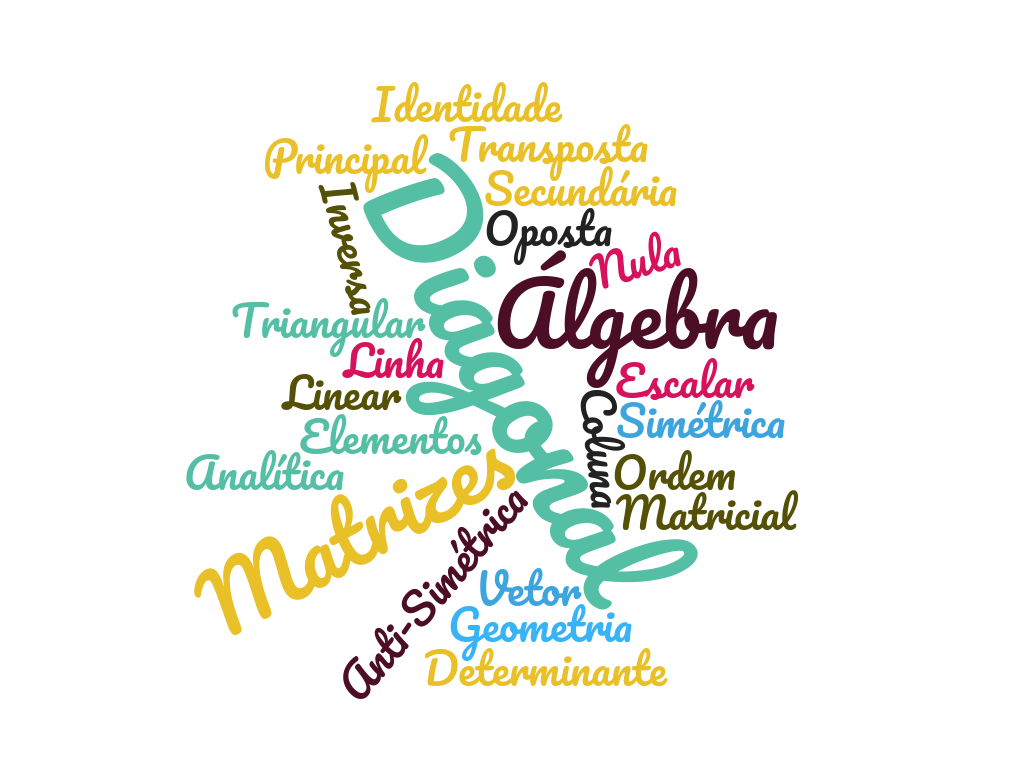
\includegraphics[scale=0.4]{linear_algebra.png}}
\end{center}
\end{figure}

\vspace{1cm}

\begin{center}
\textit{\textbf{\Large%
--- Atividade de Recuperação da Aprendizagem ---\\%
\ \\%
Outubro/2018}}
\end{center}

%\vspace{1cm}
%\begin{flushright}
%\textbf{Monitor(es):}\\
%\textit{Monitor 1\\
%Monitor 2}
%\end{flushright}

%\begin{center}
%  \fbox{\fbox{\parbox{5.5in}{\centering
%        Answer the questions in the spaces provided on the
%        question sheets. If you run out of room for an answer,
%        continue on the back of the page.}}}
%\end{center}

\end{coverpages}

\newpage

\begin{questions}
\setlength\linefillthickness{0.2pt}
%%%%%%%%%%%%%%%%%%%%%%%%%%%%%%%%%%%%%%%%%%%%%%%%%%%%%%%%%%%%%%%%%%%%%%%%%%%%%%%%%
%%%%%%%%%%%%%%%%%%%%%%%%%%%%%%%%%%%%%%%%%%%%%%%%%%%%%%%%%%%%%%%%%%%%%%%%%%%%%%%%%
%%%%%%%%%%%%%%%%%%%%%%%%%%%%%%%%%%%%%%%%%%%%%%%%%%%%%%%%%%%%%%%%%%%%%%%%%%%%%%%%%
\fullwidth{\section{Matrizes}}
%\ifprintanswers
%\newpage
%\else
%\newpage
%\fi

\question
Escreva a matriz $C = (c_{ij})_{4 \times 1}$, onde $c_{ij} = i^2 + j$.

\question
Escreva a matriz $A = (a_{ij})_{2 \times 3}$, onde:
$a_{ij} =
    \begin{cases}
      2i + j & \text{se}\ i \ge j\\
      i - j  & \text{se}\ i < j
    \end{cases}
$

\question
Chama-se \emph{traço} de uma matriz quadrada a soma dos elementos da
diagonal principal. Determine o traço de cada uma das matrizes:\\%
$A = \begin{pmatrix}
  1 & 2\\
  4 & 3\\
\end{pmatrix}$

$B = \begin{pmatrix}
  2 & 0 & 1\\
  \sqrt{2} & 3 & -5\\
  -1 & 0 & -1\\
\end{pmatrix}$

\question
Data a matriz
$A = \begin{pmatrix}
  1 & 2\\
  -1 & -4\\
\end{pmatrix}$, determine:
\begin{itemize}
\item[a.] A transposta de $A$
\item[b.] A oposta de $A$
\end{itemize}

\question
Dadas as matrizes $A = (a_{ij})_{6 \times 4}$, tal que $a_{ij} = i - j$, $B = (b_{ij})_{4 \times 5}$,
tal que $b_{ij} = j - i$, e $C = AB$, determine o elemento $c_{42}$.


%%%%%%%%%%%%%%%%%%%%%%%%%%%%%%%%%%%%%%%%%%%%%%%%%%%%%%%%%%%%%%%%%%%%%%%%%%%%%%%%%
%%%%%%%%%%%%%%%%%%%%%%%%%%%%%%%%%%%%%%%%%%%%%%%%%%%%%%%%%%%%%%%%%%%%%%%%%%%%%%%%%
%%%%%%%%%%%%%%%%%%%%%%%%%%%%%%%%%%%%%%%%%%%%%%%%%%%%%%%%%%%%%%%%%%%%%%%%%%%%%%%%%
\fullwidth{\section{Determinantes}}

\question
(FEI-SP) As faces de um cubo foram numeradas de 1 a 6; depois, em cada face, foi
registrada uma matriz de ordem 2, com elementos definidos por
$a_{ij} =
    \begin{cases}
      2i + f & \text{se}\ i = j\\
      j      & \text{se}\ i \ne j
    \end{cases}
$, onde $f$ é o valor associado à face correspondente. Qual o valor do determinante
da matriz registrada na face $5$?

\question
Seja $S = (s_{ij})$ a matriz de ordem $3$ em que
$s_{ij} =
\begin{cases}
  0     & \text{se}\ i < j\\
  i + j & \text{se}\ i = j\\
  i - j & \text{se}\ i > j
\end{cases}
$. Calcule o determinante de S.

\question
(FUVEST-SP) Calcule
$\begin{vmatrix}
  1 & 1 & 1 & 1\\
  1 & 2 & 2 & 2\\
  1 & 2 & 3 & 3\\
  1 & 2 & 3 & 4\\
\end{vmatrix}$

\question
Calcule os determinantes usando Chio e Laplace:
\begin{itemize}
\item[a.]
$\begin{vmatrix}
  2 &  3 & -1 & 0\\
  4 & -2 &  1 & 3\\
  1 & -5 &  2 & 1\\
  0 &  3 & -2 & 6\\
\end{vmatrix}$  
\item[b.]
$\begin{vmatrix}
  2 &  3 & 0 & -1\\
  5 & -6 & 2 &  4\\
  2 & -1 & 0 &  3\\
  3 &  2 & 1 &  5\\
\end{vmatrix}$
\end{itemize}


%%%%%%%%%%%%%%%%%%%%%%%%%%%%%%%%%%%%%%%%%%%%%%%%%%%%%%%%%%%%%%%%%%%%%%%%%%%%%%%%%
%%%%%%%%%%%%%%%%%%%%%%%%%%%%%%%%%%%%%%%%%%%%%%%%%%%%%%%%%%%%%%%%%%%%%%%%%%%%%%%%%
%%%%%%%%%%%%%%%%%%%%%%%%%%%%%%%%%%%%%%%%%%%%%%%%%%%%%%%%%%%%%%%%%%%%%%%%%%%%%%%%%
\fullwidth{\section{Sistemas de Equações Lineares}}

\question
Resolva o sistema:
$\begin{cases}
  x + y + 2z = -1\\
  4x + y + 4z = -2\\
  2x - y - 2z = -4
\end{cases}$

\question
Resolva o sistema utilizando Gauss:
$\begin{cases}
  x + y + z + t = 0\\
  2x - y + t = 1\\
  y + z - 2t = 0\\
  4y + 3z = 7
\end{cases}$

\question
Resolva o sistema utilizando a Regra de Cramer:
$\begin{cases}
  x + 2y - z = -1\\
  2x + y + z = 4\\
  x - y + 5z = 5
\end{cases}$

\question
(UFU-MG) Um sitiante utiliza milho, farelo de trigo e alfafa para
alimentar seus porcos. O número de unidades de cada tipo de ingrediente
nutricional básico encontrado num quilo de cada alimento é dado na
tabela abaixo, juntamente com as necessidades diárias de cada porco:

\begin{table}[h]
\centering
\begin{tabular}{@{}lccc@{}}
\toprule
\textbf{Ingredientes}    & \multicolumn{1}{l}{\textbf{Carboidratos}} & \multicolumn{1}{l}{\textbf{Proteínas}} & \multicolumn{1}{l}{\textbf{Vitaminas}} \\ \midrule
Quilo de milho           & 40                                        & 30                                     & 10                                     \\
Quilo de farelo de trigo & 20                                        & 40                                     & 20                                     \\
Quilo de alfafa          & 20                                        & 40                                     & 40                                     \\
Necessidade diária       & 110                                       & 120                                    & 70                                     \\ \bottomrule
\end{tabular}
\end{table}

Determine quantos quilos de milho, farelo de trigo e alfafa cada porco deve
consumir por dia para satisfazer suas necessidades de nutrientes.




%%%%%%%%%%%%%%%%%%%%%%%%%%%%%%%%%%%%%%%%%%%%%%%%%%%%%%%%%%%%%%%%%%%%%%%%%%%%%%%%%
%%%%%%%%%%%%%%%%%%%%%%%%%%%%%%%%%%%%%%%%%%%%%%%%%%%%%%%%%%%%%%%%%%%%%%%%%%%%%%%%%
%%%%%%%%%%%%%%%%%%%%%%%%%%%%%%%%%%%%%%%%%%%%%%%%%%%%%%%%%%%%%%%%%%%%%%%%%%%%%%%%%
%%%%%%%%%%%%%%%%%%%%%%%%%%%%%%%%%%%%%%%%%%%%%%%%%%%%%%%%%%%%%%%%%%%%%%%%%%%%%%%%%
%%%%%%%%%%%%%%%%%%%%%%%%%%%%%% TERMINA O DOCUMENTO %%%%%%%%%%%%%%%%%%%%%%%%%%%%%%
%%%%%%%%%%%%%%%%%%%%%%%%%%%%%%%%%%%%%%%%%%%%%%%%%%%%%%%%%%%%%%%%%%%%%%%%%%%%%%%%%
%%%%%%%%%%%%%%%%%%%%%%%%%%%%%%%%%%%%%%%%%%%%%%%%%%%%%%%%%%%%%%%%%%%%%%%%%%%%%%%%%
%%%%%%%%%%%%%%%%%%%%%%%%%%%%%%%%%%%%%%%%%%%%%%%%%%%%%%%%%%%%%%%%%%%%%%%%%%%%%%%%%
%%%%%%%%%%%%%%%%%%%%%%%%%%%%%%%%%%%%%%%%%%%%%%%%%%%%%%%%%%%%%%%%%%%%%%%%%%%%%%%%%
\end{questions}
\end{document}
